\documentclass[sigconf]{acmart}

\usepackage{booktabs} % For formal tables

\usepackage{amsmath}
\usepackage{float}
\usepackage{hyperref}
\usepackage{listings}
\usepackage{algorithm}
\usepackage[noend]{algpseudocode}
\usepackage{graphicx}
\usepackage{courier}
\usepackage{float}
\usepackage{color}
\usepackage[margin=10pt,font=small,labelfont=bf,
  labelsep=endash]{caption}
\usepackage{ulem}

\usepackage{syntax} % for writing BNF grammar

\usepackage{forest}
\usepackage{framed}

\usepackage{tikz}
\usetikzlibrary{matrix}
\usetikzlibrary{shapes.multipart}
\usetikzlibrary{patterns}
\usetikzlibrary{positioning,fit,calc}
\usetikzlibrary{decorations.pathmorphing}
\usetikzlibrary{decorations.pathreplacing}
\usetikzlibrary{quotes}
\usetikzlibrary{graphs}
\usetikzlibrary{arrows.meta}
\usetikzlibrary{shapes}
% \usetikzlibrary{graphs,graphdrawing}
% \usegdlibrary{layered}
% \usetikzlibrary{graphdrawing,graphs,calc}
% \usegdlibrary{layered}

\usepackage{smartdiagram}

% \usetikzlibrary{external}
% \tikzexternalize % activate!
% \tikzset{external/force remake}

%% To generate figure, uncomment above three lines, and execute:
%% pdflatex -shell-escape helium.tex

\usepackage{csvsimple}
\usepackage{multirow}


\lstset{basicstyle=\footnotesize\ttfamily,breaklines=true}
% \lstset{frame=b}
\lstset{float,floatplacement=H,captionpos=b}
% \lstset{numbers=left}
\lstset{language=C}
\lstset{showstringspaces=false}
\lstset{breakindent=10pt}
% \lstset{framextopmargin=10pt}
% \lstset{framextopmargin=50pt,frame=t}
% \lstset{float=htb,language=C,frame=single, basicstyle=\small, stringstyle=\ttfamily}
% \lstset{escapeinside={(*@}{@*)}}
% \usepackage{xcolor}
\lstdefinestyle{base}{
  language=C,
  emptylines=1,
  breaklines=true,
  aboveskip=0em,
  belowskip=0em,
  % float,
  % floatplacement=H,
  basicstyle=\footnotesize\ttfamily\color{black},
  moredelim=**[is][\color{blue}]{@}{@},
  moredelim=**[is][\color{purple}]{~1}{~1},
  moredelim=**[is][\color{brown}]{~2}{~2},
  moredelim=**[is][\color{gray}]{~3}{~3},
  moredelim=**[is][\color{orange}]{~4}{~4},
  moredelim=**[is][\color{violet}]{~5}{~5},
}
\lstdefinestyle{graycode} {
  language=C,
  emptylines=1,
  breaklines=true,
  basicstyle=\footnotesize\ttfamily\color{gray!50},
  moredelim=**[is][\color{blue}]{@}{@},
}
\begin{document}





\title{Figures}

This is figure 1.

\begin{figure*}[h!]
  \centering
  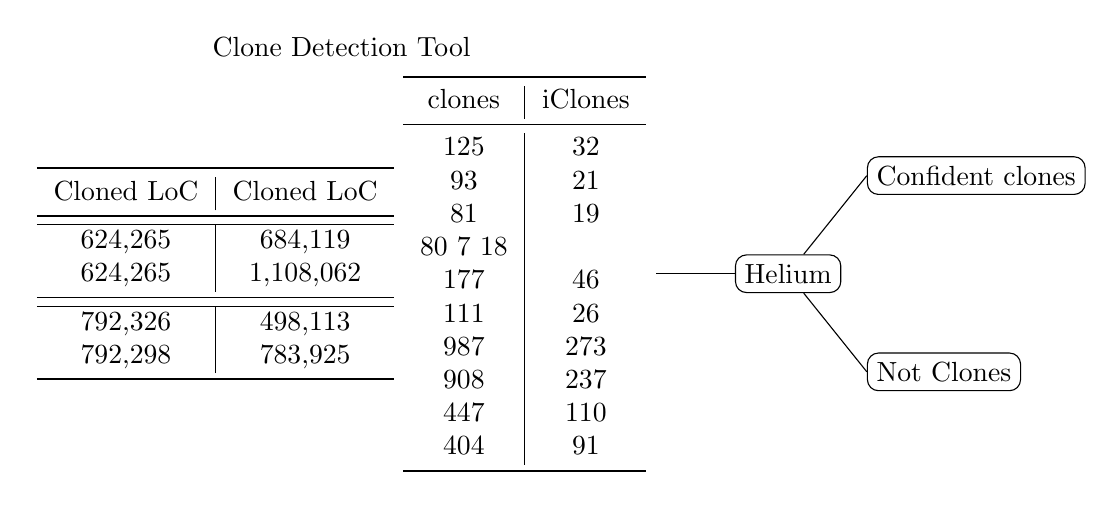
\begin{tikzpicture}

    % \matrix[] (whole) {
    %     \matrix[] (inner) {
    %       \node {Hello};&
    %       \node {World};\\
    %     };&
    %   \node {Delta Debugging};\\
    %   \node {IDE};&
    %   \node {Bug Signature};\\
    % };

    \node (tool) ["Clone Detection Tool"] {
      \begin{tabular}{c | c}
        \toprule
        Cloned LoC & Cloned LoC\\
        \midrule\hline
        624,265 & 684,119\\
        624,265 & 1,108,062\\
        \midrule\hline
        792,326 & 498,113\\
        792,298 & 783,925\\
        \bottomrule
      \end{tabular}

      \begin{tabular}{c|c}
        \toprule
        clones & iClones \\
        \midrule
        125& 32\\
        93& 21\\
        81 & 19\\
        80 7 18\\
        177 & 46\\
        111 & 26\\
        987 & 273\\
        908 & 237\\
        447 & 110\\
        404 & 91\\
        \bottomrule
      \end{tabular}
    };
    \node (helium) [draw, rounded corners, right=of tool] {Helium};
    \node (conf-clone) [draw, rounded corners,
      right=of helium.north, shift={(0,1)}] {Confident clones};
    \node (not-clone) [draw, rounded corners,
      right=of helium.south, shift={(0,-1)}] {Not Clones};

    \draw (tool) -- (helium);
    \draw (helium) -- (conf-clone.west);
    \draw (helium) -- (not-clone.west);
    

  \end{tikzpicture}
\end{figure*}

\begin{figure*}
  \centering
  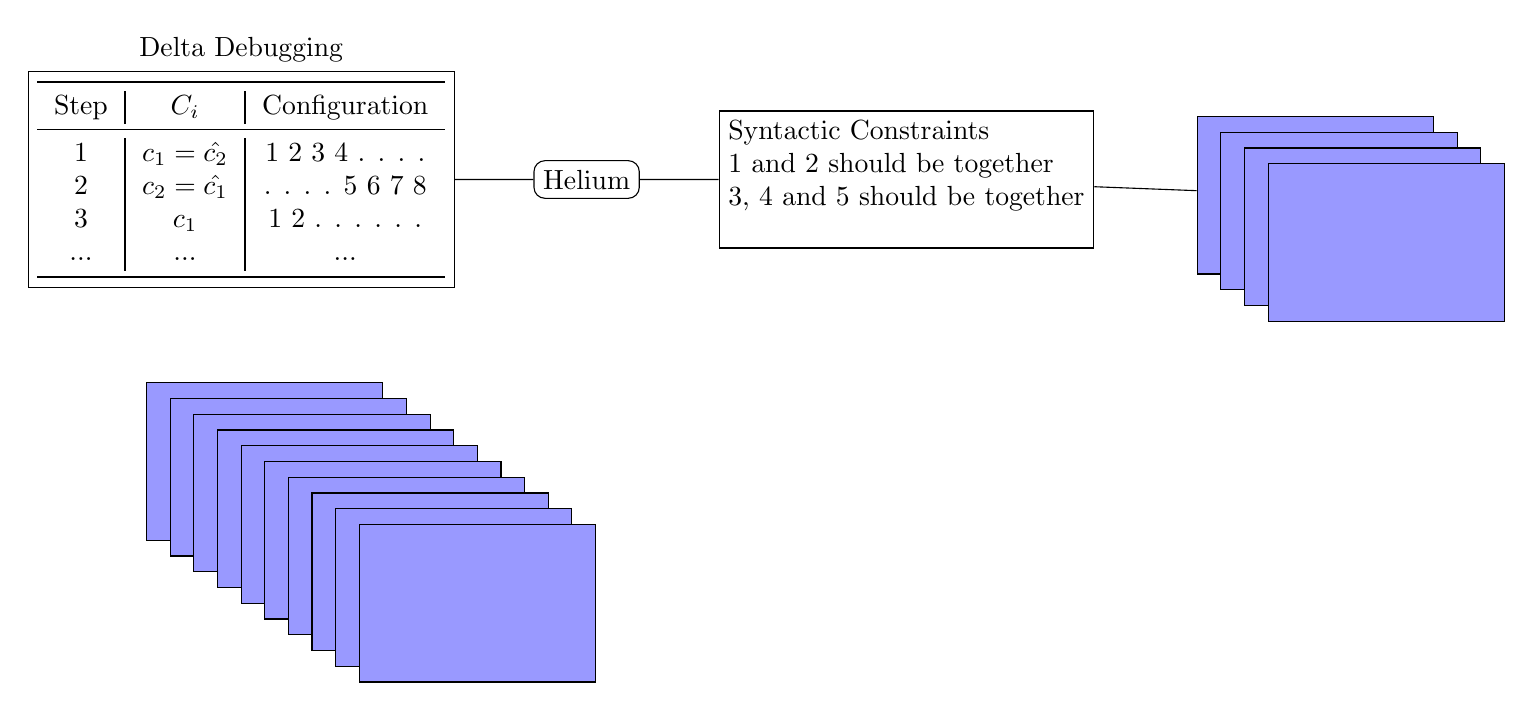
\begin{tikzpicture}
    \node (delta) [draw, "Delta Debugging"] {
      % # a table
      \begin{tabular}{c | c | c}
        
        \toprule
        Step & $C_i$ & Configuration \\
        \midrule
        1 & $c_1 = \hat{c_2}$ & 1 2 3 4 . . . .\\
        2 & $c_2 = \hat{c_1}$ & . . . . 5 6 7 8\\
        3 & $c_1$ &             1 2 . . . . . .\\
        ... & ... & ... \\
        \bottomrule

      \end{tabular}
      % # some visualization
      % \node [draw,
      %   % minimum width=2.2cm,minimum height=2.5cm
      %   % minimum width=3cm, minimum height=3cm
      %   ]{Hello World};

      % \node (innnn) {Hello};
      
    };
    \begin{scope}[every node/.style=draw, minimum width=3cm, minimum height=2cm]
      \foreach \x in {1, 2, 3, 4, 5, 6, 7, 8, 9, 10}
      \node (in-\x) [below=of delta, fill=blue!40, shift={(\x * 0.3 cm, - \x * 0.2 cm)}] {};
    \end{scope}
    
    \node (helium) [draw, rounded corners, right=of delta] {Helium};
    \node (constraint) [draw, right=of helium, align=left] {
      Syntactic Constraints\\
      1 and 2 should be together\\
      3, 4 and 5 should be together\\
    };
    % \node (output) [draw, right=of constraint] {Output};

    \begin{scope}[every node/.style=draw, minimum width=3cm, minimum height=2cm]
      \foreach \x in {1, 2, 3, 4}
      \node (output-\x) [right=of constraint, fill=blue!40, shift={(\x * 0.3 cm, - \x * 0.2 cm)}] {};
    \end{scope}
    

    \draw (delta) -- (helium) -- (constraint) -- (output-1);

    
  \end{tikzpicture}

\end{figure*}

\begin{figure*}
  \centering
  \begin{tikzpicture}
    \node (ide) [draw, minimum width=10cm, minimum height=6cm] {IDE};
    % IDE should have menu
    % IDE should support selection of nodes
    % IDE should output something
    \node (out1) [draw, rounded corners, anchor=north, right=of ide.north east] {Output 1};
    \node (out2) [draw, rounded corners, below=of out1] {Output 2};
    \node (out3) [draw, rounded corners, below=of out2] {Output 3};
    \node (out4) [draw, rounded corners, below=of out3] {Output 4};


    
    
  \end{tikzpicture}

\end{figure*}



\end{document}
